\documentclass{article}

\usepackage{tabularx}

% NOTE: To put equations in their environment we need either `float` or
% `caption`.  We use float to put equations and other environments exactly
% where they appear in the code with the `H` placeholder, and for that we
% redefine the `equ` environment sort of twice, so this is a bit flaky but
% it works.
\usepackage{caption}
\usepackage{subcaption}

\DeclareCaptionType{equ}[][]
\captionsetup[equ]{name=נוסחא}
\usepackage{float}
\floatstyle{plain}
% https://www.overleaf.com/learn/latex/Positioning_of_Figures
\newfloat{equ}{H}{eq}[section]
\floatname{equ}{נוסחא}

\DeclareCaptionType{graph}[][]
\captionsetup[graph]{name=גרף }

\usepackage{physics}

% to includegraphics
\usepackage{graphicx}

% to fix itemize lists:
% https://tex.stackexchange.com/a/53453/125609
\usepackage{enumitem}
\setlist[itemize,1]{label={\fontfamily{cmr}\fontencoding{T1}\selectfont\textbullet}}

% To crop inserted images: https://tex.stackexchange.com/questions/57418/crop-an-inserted-image
\usepackage[export]{adjustbox}

% For hbar
\usepackage{unicode-math}
%\setmathfont{Stix Two Math}

% Links
\usepackage{hyperref}
\hypersetup{colorlinks = true,
	citecolor = gray,
	linkcolor = red,
	citecolor = green,
	filecolor = magenta,
	urlcolor = cyan
}

\usepackage[version=4]{mhchem}

% To include plots by matplotlib
\usepackage{pgf}
\usepackage{pgfplots}
\pgfplotsset{compat=newest}
% Note we use resizebox as explained here through out the document https://tex.stackexchange.com/a/582956/125609

\usepackage{geometry}
 \geometry{
 a4paper,
 top=30mm,
 left = 25mm,
 right = 25mm,
 bottom=30mm,
 headheight=2cm,
 headsep=2cm,
 footskip=1.5cm
}

% Language
\usepackage{polyglossia}
\setdefaultlanguage{hebrew}
\setotherlanguage{english}
\usepackage{hebrewcal}

\usepackage[
backend=biber,
isbn=false,
style=numeric,
doi = false,
sorting=ynt
]{biblatex}
% Seems to be a recommended package but it makes quotes in bibliography at the
% end appear with a question mark instead of `"`.
%\usepackage{csquotes}
\addbibresource{references.bib} % Imports bibliography file

% Fonts
\setmainfont{David CLM}
\setsansfont{Libertinus Serif}
\setmonofont{FreeMono}
\newfontfamily\hebrewfont{David CLM}[Script=Hebrew]
\newfontfamily\hebrewfontsf{Libertinus Serif}[Script=Hebrew]
\newfontfamily\hebrewfonttt{FreeMono}[Script=Hebrew]

\title{
	% TODO
} 
\author{
שרה לחצר ודורון בכר \\
הפקולטה לפיזיקה, טכניון - מכון טכנולוגי לישראל.
}
\date{\today}

\begin{document}
\maketitle

\begin{abstract}
	% TODO
\end{abstract}

\section{
מבוא
}
 בטבע קיימים יסודות הפולטים באופן ספונטני חלקיקים מגרעין האטום שלהם. פליטה ספונטנית זו נקראת קרינה רדיואקטיבית. קרינה זו גורמת לגרעין
להיות יציב יותר על ידי הקטנת אנרגיית הגרעין באמצעות פליטה של חלקיקים אנרגטיים ממנו.
ישנם מספר סוגים של קרינה רדיואקטיבית שמסווגים לפי סוג החלקיקים הנפלטים מהגרעין.
ניסוי זה מתמקד בקרינה רדיואקטיבית מסוג 
$\alpha$
ו-
$\beta$.

כידוע חלקיקים העוברים דרך חומר מאבדים אנרגיה כתוצאה מהתנגשויות עם האטומים בחומר.
נרצה לבחון את המרחק שעובר חלקיק בחומר עד שהוא מאבד את מרבית האנרגיה שלו.
ההתנהגות התאורטית עבור חלקיק ה- 
$\alpha$
מוצגת באיור
\ref{fig:alphaDecay}.

\begin{figure}[ht!]
    \centering
    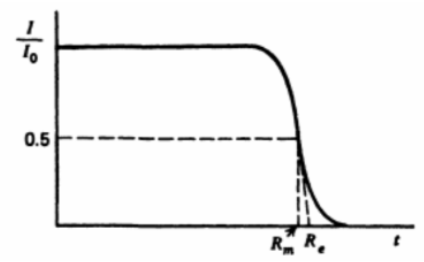
\includegraphics{alphaRadiation.png}
    \caption{
    אופיין איכותי של התנהגות עוצמת קרינת 
    $\alpha$
    במעבר בחומר ביחס למרחק.
    %TODO: explain R_m and R_e
    }
    \label{fig:alphaDecay}
\end{figure}

בנוסף
מדדנו את את הקשר בין עוצמת הקרינה למרחק מהגלאי.
כאשר הקשר התאורטי ניתן בנוסחא 
\ref{equ:distanceIntensity}.

\begin{equ}
$$I(r) = \frac{I_0}{r^2}$$
\caption{
היחס בין עוצמת הקרינה למרחק מן הגלאי עבור 
$I_0$ 
העוצמה המקסימלית.
}
\label{equ:distanceIntensity}
\end{equ}

חלקיקי ה
$\beta$
הם אלקטרונים שנפלטים מהאטום כאשר ניוטרון דועך והופך לניטרון אלקטרון וניוטרנו.
גם עבור חלקיק ה
$\beta$
נרצה למדוד את הדעיכה בעת מעבר דרך חומר.
בעזרת חוק
\textenglish{Beer-Lambert}
נוכל לקבל את היחס בין העוצמה לעובי החומר .

\begin{equ}
$$I = I_0 e^{-\mu t}$$
\caption{עוצמת הקרינה כתלות בעובי החומר בה היא עוברת כאשר
$\mu$
מקדם הדעיכה}
\end{equ}
\clearpage
\section{
מערכת הניסוי
}
מערכת הניסוי מוצגת באיור 
\ref{fig:systemSetupNuclear}.
המערכת מורכבת ממונה גייגר, אפליקציה שבעזרתה ניתן למדוד את מספר הקריאות שהמונה קיבל בזמן נתון,
וחוסמי קרינה מסוגים ועוביים שונים.

% TODO: add ref to the guide
\begin{figure}[ht!]
    \centering
    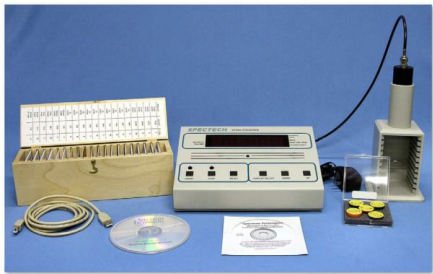
\includegraphics{systemSetup.png}
    \caption{
    מערכת הניסוי.
    \cite{Manual}
    }
    \label{fig:systemSetupNuclear}
\end{figure}

מונה גייגר בנוי משפופרת גלילית מוליכה בעלת חלון כניסה דק. השפופרת משמשת כקתודה ומכילה בתוכה אנודה העשויה מחוט מוליך הנמצא במתח גבוה ומבודד מהדפנות.
בתוך השפורפרת מצוי גז אציל, כך בעת כניסת קרינה לתא היא מיננת את הגז.
המטען נאסף בתיל החיובי, וכאשר הוא זורם חזרה לדפנות, נרשמת במערכת פעימה שמעידה על אירוע. המכשיר מגביר את האות ומציג אותו למשתמש.

לאחר היינון חלה רגיעה,
האלקטרונים והאטומים מתלכדים מחדש בזמן המכונה זמן ההתלכדות. בטווח זמנים זה המכשיר אינו מסוגל להוציא אותות נוספים.

כיוצא מן הכתוב, כמות הפעימות תלויה במתח המסופק. בגרף
\ref{fig:plateau}
מוצג יחס זה.

\begin{figure}[ht!]
    \centering
    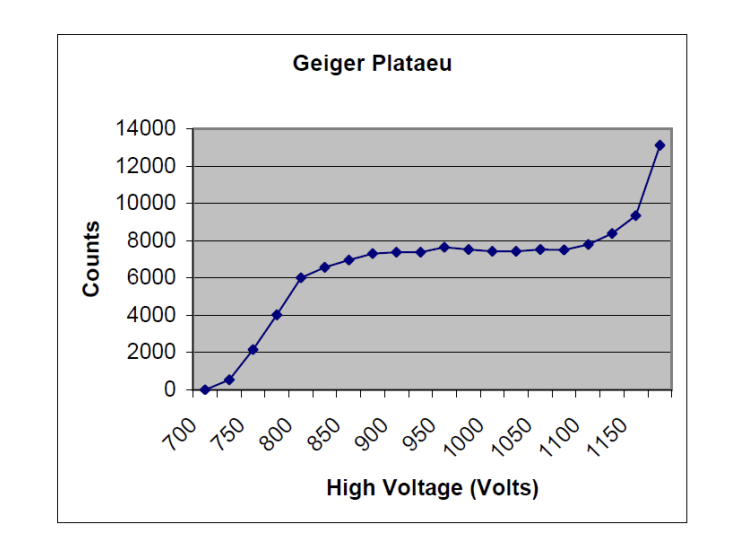
\includegraphics{plateau.png}
    \caption{כמות הפעימות כתלות במתח במונה גייגר, לקוח מהתדריך}
    \label{fig:plateau}
\end{figure}

מתח העבודה הרצוי יהיה בתחום ה
\textenglish{"plateau"},
בו כמות הפעימות בקירוב איננה משתנה כתלות במתח.

\section{
תוצאות
}

\subsection{
מדידת דעיכת בטא
}

% TODO: Explain this

\begin{figure}[ht!]
    \centering
    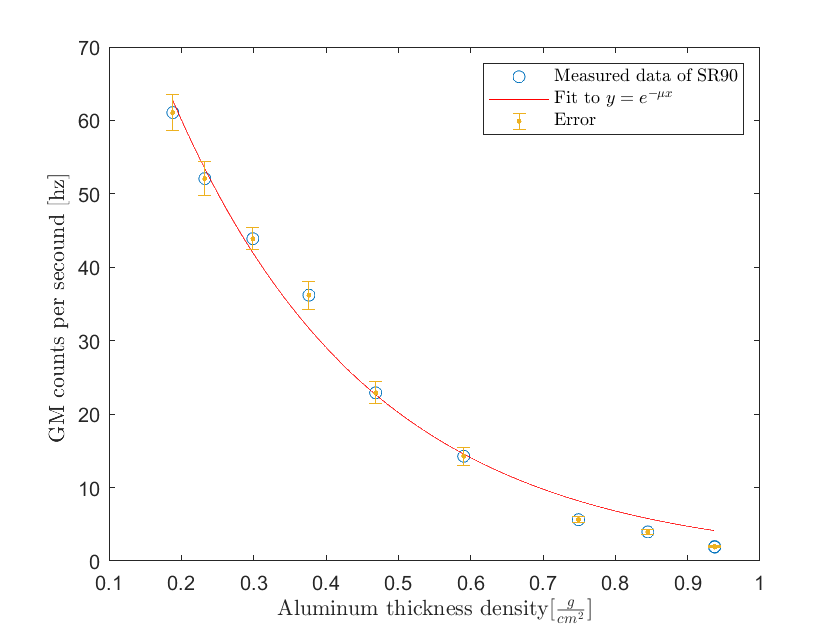
\includegraphics[width=0.79\textwidth]{SR90.png}
    \caption{Caption}
    \label{fig:decay_SR90}
\end{figure}

\begin{figure}[ht!]
    \centering
    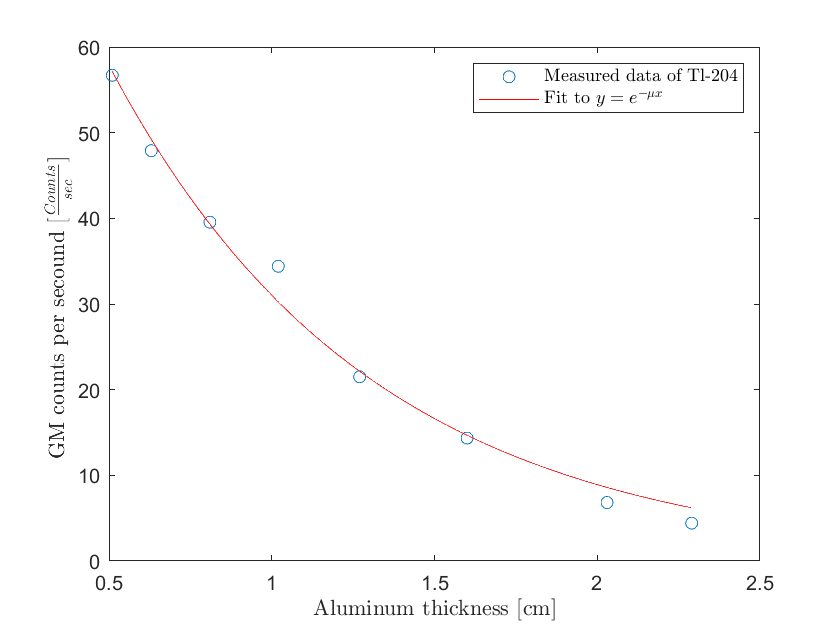
\includegraphics[width=0.79\textwidth]{Tl-204.png}
    \caption{Caption}
    \label{fig:decay_Tl-204}
\end{figure}

\subsection{
מדידת דעיכת עוצמת קרינה כתלות במרחק
}

עבור
\textenglish{Thalium-204}
ועבור
\textenglish{Strontium-90}
מדדנו את הקשר בין עוצמת הקרינה הרדיואקטיבית למרחק של המקור הרדיואקטיבי מהגלאי. ביצענו התאמה לביטוי דומה לביטוי במשוואה
\ref{equ:distanceIntensity}:

\begin{equ}
$$ I(r) \sim \frac{1}{(r+a)^2}$$
\label{equ:distanceIntensity_fit}
\end{equ}

ביצענו התאמה לפונקציה זו כי לא הייתה באפשרותינו למדוד את המרחק בין המקור לגלאי באופן אבסולוטי, אלא רק באופן יחסי. התוצאות מוצגות בגרפים

\begin{graph}
\includegraphics[]{}
\end{graph}

\section{
דיון בתוצאות
}

\section{
מסקנות
}

\section*{
סימוכין
}

\begin{english}
\printbibliography[heading=none]
\end{english}

\end{document}
